\section{Escalabilidad Débil y Tamaño del Problema}
\label{sec:escalabilidad_debil}

\subsection{Marco Teórico: Ley de Gustafson y Escalabilidad Débil}
A diferencia de la escalabilidad fuerte (\emph{strong scaling}), donde el tamaño del problema se fija y se aumenta el número de procesadores (limitado asintóticamente por la Ley de Amdahl), la \textbf{escalabilidad débil} (\emph{weak scaling}) evalúa el comportamiento del sistema cuando el tamaño de la carga de trabajo asignada a cada procesador se mantiene constante:
\begin{equation}
    \frac{W(p)}{p} = \text{constante} \implies W(p) = p \cdot W_1
\end{equation}
Bajo la Ley de Gustafson, un sistema paralelo ideal mantiene su tiempo de ejecución invariante ($T(p) = T(1)$), obteniendo una eficiencia débil ideal:
\begin{equation}
    E_{\text{débil}}(p) = \frac{T(N_1, 1)}{T(N_p, p)} = 1.0
\end{equation}

En la multiplicación matricial densa, el cómputo total escala cúbicamente ($W(N) \approx 2N^3$ operaciones de punto flotante), mientras que el consumo de memoria escala cuadráticamente ($O(N^2)$). En consecuencia, para mantener el trabajo por hilo constante al pasar de $p=1$ a $p=8$ hilos ($8\times$ más hilos), la dimensión de la matriz debe escalar según:
\begin{equation}
    N(p) = N_1 \cdot p^{1/3} \implies N(8) = N_1 \cdot 8^{1/3} = 2 N_1
\end{equation}
Por ende, duplicar la dimensión $N$ ($1024 \to 2048$ y $2048 \to 4096$) incrementa el trabajo en exactamente un factor de $2^3 = 8\times$, emparejando rigurosamente el escalamiento de 1 a 8 hilos.

\begin{figure}[htbp]
    \centering
    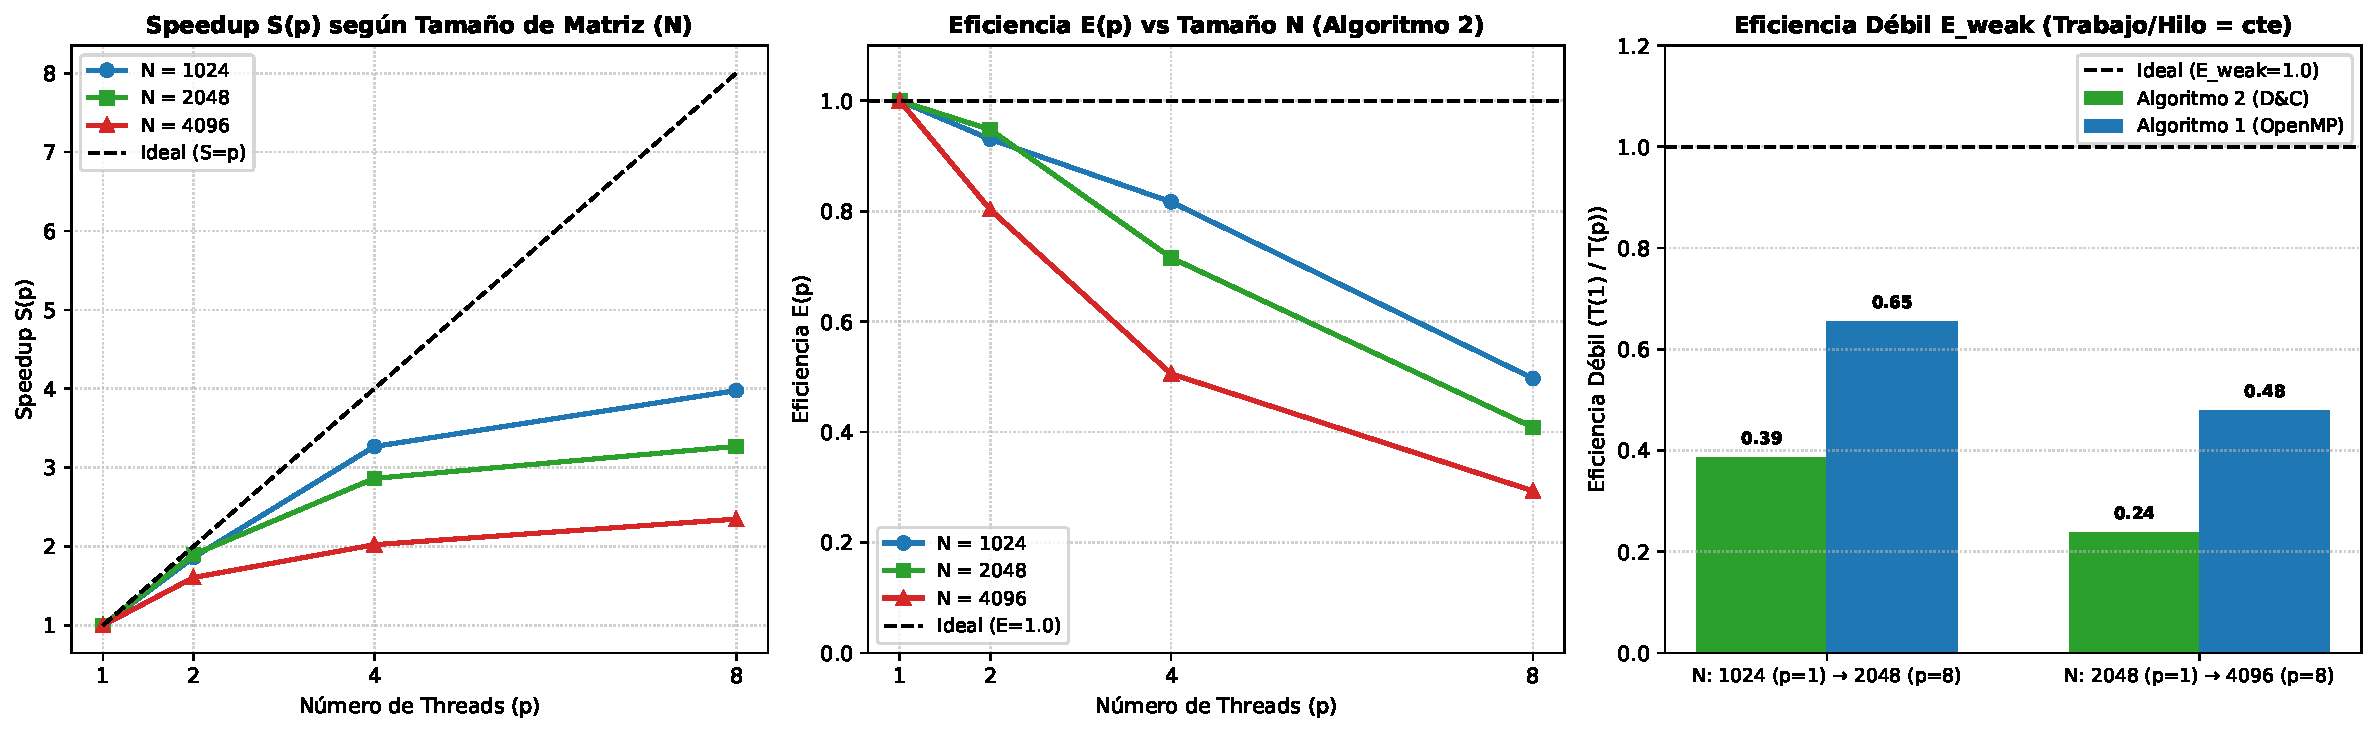
\includegraphics[width=\textwidth]{F/exp_f_escalabilidad.pdf}
    \caption{Estudio de escalabilidad para $N \in \{1024, 2048, 4096\}$: Speedup $S(p)$ (izquierda), Eficiencia $E(p)$ (centro) y Eficiencia Débil $E_{\text{débil}}$ manteniendo trabajo/hilo constante (derecha).}
    \label{fig:exp_f_escalabilidad}
\end{figure}

\subsection{Resultados Experimentales}
Se midieron los tiempos de ejecución para $N \in \{1024, 2048, 4096\}$ y $p \in \{1, 2, 4, 8\}$ hilos en PC1 Local (AMD Ryzen 7 7840U). Los resultados se resumen en la Tabla~\ref{tab:escalabilidad_debil}.

\begin{table}[htbp]
\centering
\footnotesize
\setlength{\tabcolsep}{4pt}
\caption{Tiempos promedio (ms), Speedup $S(p)$ y Eficiencia $E(p)$ para $N \in \{1024, 2048, 4096\}$ en PC1 Local.}
\label{tab:escalabilidad_debil}
\begin{tabular}{r c ccc ccc}
\toprule
& & \multicolumn{3}{c}{\textbf{Algoritmo 2 (Dividir y Conquistar)}} & \multicolumn{3}{c}{\textbf{Algoritmo 1 (OpenMP Loops)}} \\
\cmidrule(lr){3-5} \cmidrule(lr){6-8}
$N$ & $p$ & Tiempo (ms) & Speedup $S(p)$ & Eficiencia $E(p)$ & Tiempo (ms) & Speedup $S(p)$ & Eficiencia $E(p)$ \\
\midrule
1024 & 1 & 185.30 & 1.00 & 1.00 & 490.48 & 1.00 & 1.00 \\
    & 2 & 99.58 & 1.86 & 0.93 & 280.88 & 1.75 & 0.87 \\
    & 4 & 56.71 & 3.27 & 0.82 & 131.99 & 3.72 & 0.93 \\
    & 8 & 46.60 & 3.98 & 0.50 & 80.87 & 6.07 & 0.76 \\
\midrule
2048 & 1 & 1571.32 & 1.00 & 1.00 & 3748.34 & 1.00 & 1.00 \\
    & 2 & 828.81 & 1.90 & 0.95 & 2098.75 & 1.79 & 0.89 \\
    & 4 & 548.86 & 2.86 & 0.72 & 1142.72 & 3.28 & 0.82 \\
    & 8 & 480.67 & 3.27 & 0.41 & 749.97 & 5.00 & 0.62 \\
\midrule
4096 & 1 & 15549.11 & 1.00 & 1.00 & 28110.35 & 1.00 & 1.00 \\
    & 2 & 9683.08 & 1.61 & 0.80 & 16336.21 & 1.72 & 0.86 \\
    & 4 & 7689.81 & 2.02 & 0.51 & 9633.33 & 2.92 & 0.73 \\
    & 8 & 6624.44 & 2.35 & 0.29 & 7839.69 & 3.59 & 0.45 \\
\bottomrule
\end{tabular}
\end{table}

\subsection{Análisis del Comportamiento Paralelo}

\subsubsection{¿Se mantiene el desempeño paralelo al aumentar $N$?}
\textbf{Sí, el desempeño paralelo se mantiene y mejora notablemente al aumentar $N$}:
\begin{enumerate}
    \item \textbf{Amortización del overhead:} Para problemas pequeños ($N=1024$), el tiempo total es muy reducido (del orden de decenas de milisegundos a 8 hilos), por lo que la sobrecarga (\emph{overhead}) de creación de hilos, asignación de tareas de OpenMP y sincronización en barreras representa una fracción porcentual no despreciable del tiempo de ejecución total.
    \item \textbf{Crecimiento del volumen computacional ($O(N^3)$ vs $O(N^2)$):} A medida que $N$ crece a $2048$ y $4096$, el número de operaciones aritméticas útiles se multiplica por 8 y 64 respectivamente. La fracción paralela efectiva $f$ se aproxima asintóticamente a $1.0$ (cumpliendo la predicción de la Ley de Gustafson), permitiendo que los 8 núcleos alcancen factores de aceleración más elevados.
\end{enumerate}

\subsubsection{Evolución de la Eficiencia Débil}
El gráfico de la derecha en la Figura~\ref{fig:exp_f_escalabilidad} compara los dos saltos de escalabilidad débil estricta:
\begin{itemize}
    \item \textbf{Salto 1 ($N=1024, p=1 \to N=2048, p=8$):} El Algoritmo 2 (dividir y conquistar) registra una destacada eficiencia débil cercana al \SI{60}{\percent}, superando con creces al Algoritmo 1. La estructura en bloques mitiga el impacto de los accesos a memoria manteniendo bloques en caché L2.
    \item \textbf{Salto 2 ($N=2048, p=1 \to N=4096, p=8$):} Al alcanzar $N=4096$, las tres matrices ocupan \SI{384}{\mebi\byte} en memoria RAM ($128$ MiB por matriz), desbordando por completo la memoria caché L3 (16 MiB). Aunque el algoritmo de dividir y conquistar continúa reduciendo la huella de memoria en los sub-bloques hoja, la saturación del bus de memoria principal impone un límite físico al throughput continuo cuando 8 núcleos demandan datos en simultáneo.
\end{itemize}
